\documentclass[12pt, a4paper]{article}
\usepackage{amsmath,amsfonts,amssymb,amsthm,mathtools}
\usepackage{fontspec}         % пакет для подгрузки шрифтов
\setmainfont{Arial} 
\defaultfontfeatures{Mapping=tex-text}

% why do we need \newfontfamily:
% http://tex.stackexchange.com/questions/91507/
\newfontfamily{\cyrillicfonttt}{Arial}
\newfontfamily{\cyrillicfont}{Arial}
\newfontfamily{\cyrillicfontsf}{Arial}
\usepackage{unicode-math}     % пакет для установки математического шрифта
\setmathfont{Asana-Math.otf}   
\usepackage{polyglossia}
\setdefaultlanguage{russian}  % Основной язык документа
\setotherlanguage{english}   
\usepackage{graphicx}                  % Для вставки рисунков
\usepackage{graphics}
\graphicspath{{images/}{pictures/}}    % можно указать папки с картинками
\usepackage{wrapfig} 
\usepackage{tikz, pgfplots}  % язык для рисования графики из latex'a


%%%%%%%%%% Гиперссылки %%%%%%%%%%
\usepackage{xcolor}              % разные цвета
\usepackage{hyperref}
\hypersetup{
    unicode=true,           % позволяет использовать юникодные символы
    colorlinks=true,       	% true - цветные ссылки, false - ссылки в рамках
    urlcolor=blue,          % цвет ссылки на url
    linkcolor=red,          % внутренние ссылки
    citecolor=green,        % на библиографию
	pdfnewwindow=true,      % при щелчке в pdf на ссылку откроется новый pdf
	breaklinks              % если ссылка не умещается в одну строку, разбивать ли ее на две части?
}

\usepackage{csquotes}            % Еще инструменты для ссылок
\usepackage{float}

\usepackage{csquotes}  
\usepackage{setspace}
\usepackage{extsizes}
\usepackage[paper=a4paper,top=10mm, bottom=10mm,left=35mm,right=35mm,includefoot,includehead]{geometry}
\usepackage{extsizes}
\setstretch{1}  % Межстрочный интервал

\setlength{\parskip}{4mm}   % Расстояние между абзацами
\usepackage{fancyhdr} 
\pagestyle{fancy}
\begin{document}


\renewcommand{\thesection}{Приложение \Asbuk{section}}

\setcounter{section}{0}
\thispagestyle{empty}

\begin{figure}[H]
\centering

\includegraphics[height=6cm]{hg1.png}
\end{figure}

\vspace{1cm}
\begin{flushleft}
{ \fontsize{12}{1}\selectfont Мистеру Поттеру,}
\end{flushleft}
\newcommand{\newsize}[1]
{{\fontsize{14}{1}\selectfont #1 }}
\vspace{2.5cm}
\newsize{Дорогой, Мистер Поттер,}\par
\noindent
\newsize{Мы рады проинформировать Вас о том, что Вам предоставлено место в Школе Чародейства и Волшебства <<Хогвартс>>.}\par
\noindent
\newsize{Пожалуйста, ознакомьтесь с приложенным к данному письму списком необходимых книг и предметов.}\par
\noindent
\newsize{Занятия начинаются 1 сентября. Ждем Вашу сову не позднее 31 июля.}\par
\noindent
\newsize{Искренне ваша,}\par
\newsize{\fontspec{Aldine}{Minerva Mc gonagall}}\par
\noindent
\newsize{Минерва МакГонагалл}\\
\noindent
\newsize{заместитель директора}
\vfill
\begin{center}
\newsize{Школа Чародейства и Волшебства Хогвартс}\\
Директор: Альбус Дамблдор\\(Кавалер ордена Мерлина первой степени, основатель Ордена\\Феникса, председатель Международной Конфедерации Магов)\\ 
 \href{http://hogwarts.ru/}{Ссылка на сайт школы}
\end{center}






\newpage

\fancyhead[LE,LO]{\rightmark}
\fancyhead[RE,RO]{\thepage}
\fancyhead[LE,LO]{\leftmark}
\fancyfoot[C]{Школа Чародейства и Волшебства Хогвартс}
\section{Список необходимых книг и предметов}
\renewcommand{\labelitemi}{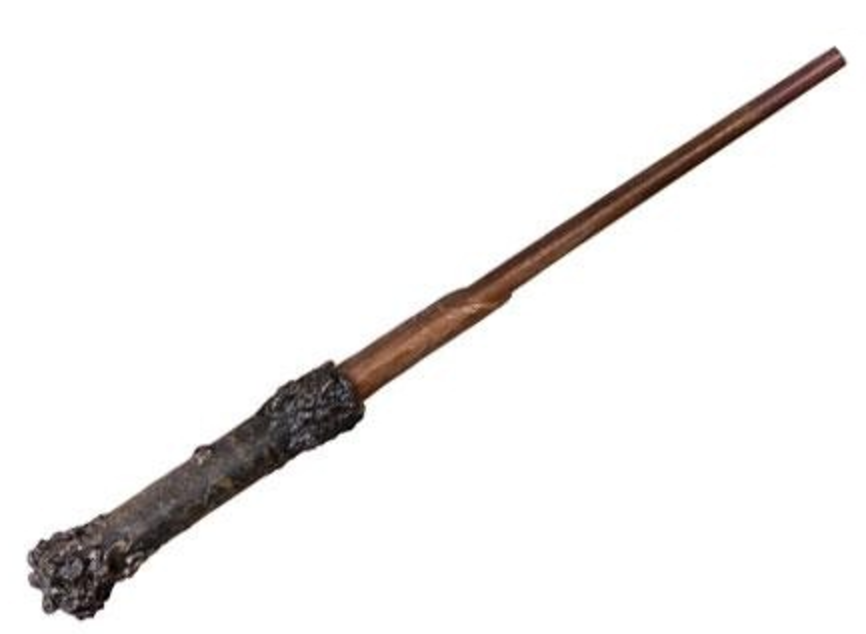
\includegraphics[scale=0.05]{mg.png}}
\begin{itemize}
\item Волшебная палочка
\item Учебник по защите от темных искусств
\item Котелок для зельеварения
\item Энциклопедия поганок

\end{itemize}
\newpage
\section{Список изучаемых предметов}
\begin{itemize}
\item Защита от темных искусств
\item Травология
\item Зельеварение
\end{itemize}


\clearpage



\end{document}